\chapter{Вычислительные эксперименты}
\section{Алгоритм решения}

Для численного решения дифференциального уравнения будем использовать алгоритм Рунге-Кутты \cite{1964calculus} четвертого порядка. 

Метод Рунге-Кутты четвертого порядка (RK4) обладает порядком точности \( O(h^4) \), что означает, что ошибка метода уменьшается пропорционально четвертой степени размера шага \( h \). Локальная ошибка на каждом шаге составляет \( O(h^5) \), а глобальная ошибка, накапливаясь после \( N \) шагов, составляет \( O(h^3) \). Это делает метод RK4 более точным по сравнению с методами более низкого порядка, такими как метод Эйлера и метод Рунге-Кутты второго порядка. Благодаря высокой точности и простоте реализации, RK4 широко используется для численного решения обыкновенных дифференциальных уравнений в различных областях науки и техники.

Результатом будет являться массив значений, каждое из которых будет являться решением дифференциального уравнения (\ref{eq:dif_temp_balance}) с заданными параметрами.

\section{Программа для ЭВМ}

В качестве языка программирования для расчётов и визуализации был выбран Python с использованием библиотек numpy (вычисления) и matplotlib (визуализация).

\lstinputlisting[language=Python,
captionpos=t,
]{../Heater.py} 

Класс SolderingIron возвращает массив значений численного решения.

\newpage
\section{Модели без терморегулятора}

Построим решения нескольких моделей для нагревателя без использования терморегулятора.

\begin{figure}[h]  % Окружение для картинки
	\centering
	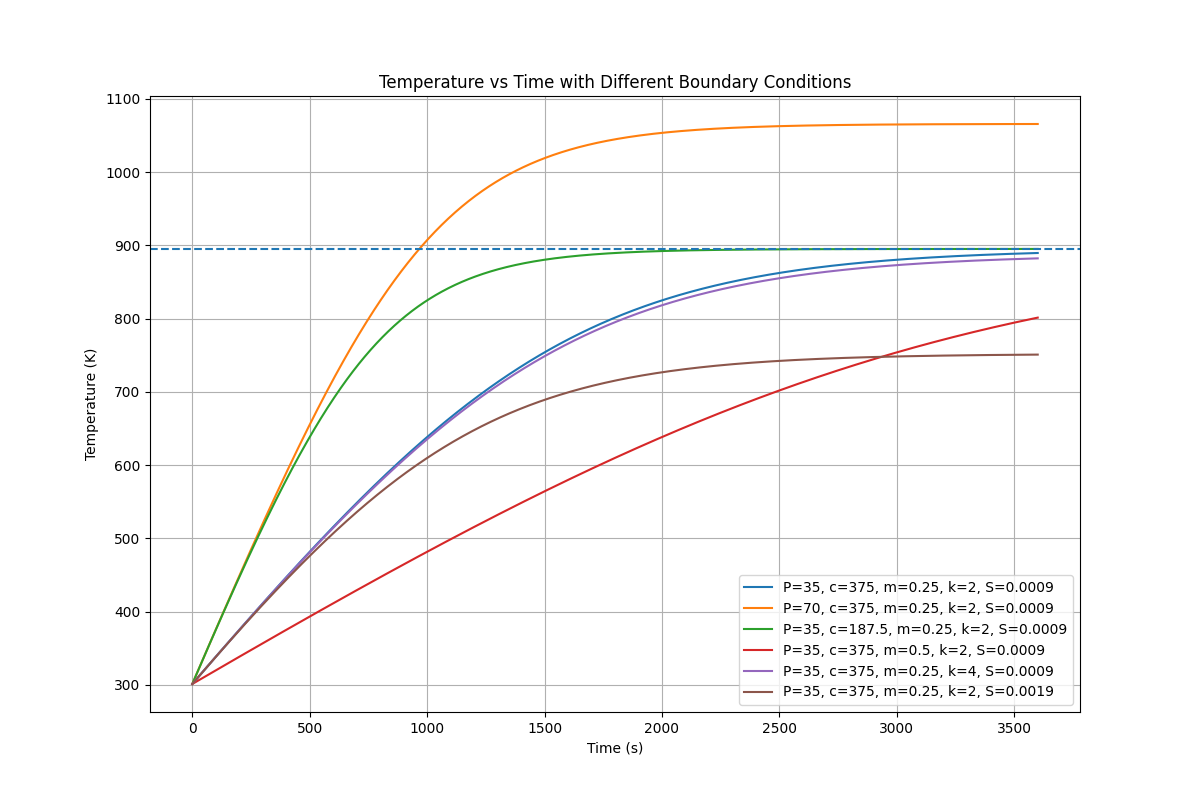
\includegraphics[width=1\textwidth]{imgs/heater_w.o_controll.png}  % Вставка изображения
	\caption{Моделирование для $T_0 = 301$.}  % Подпись к изображению
	\label{fig:heater_without_controll}  % Метка для ссылки
\end{figure}

На рис. \ref{fig:heater_without_controll} изображены графики решений при разных параметрах, которые указаны в легенде графика. Также отмечена теоретически предсказанная максимальная температура при параметрах из предыдущей главы $T = 895.53$.

Заметим, что два графика, у которых меняется только масса и удельная теплоёмкость, возрастают до предсказанной точки равновесия.

Остальные же отличаются в параметрах, влияющих на точку равновесия. Для них, это значение тоже можно увидеть.

\section{Модели с терморегулятором}

Построим решения уравнения с терморегулятором для моделей с разными параметрами.
Каждый рисунок - изображение решения уравнения \ref{eq:dif_temp_balance_with_switcher} с одним набором параметров, но разными минимальными и максимальными температурами, отмеченными пунктиром.
\begin{figure}[h]  % Окружение для картинки
	\centering
	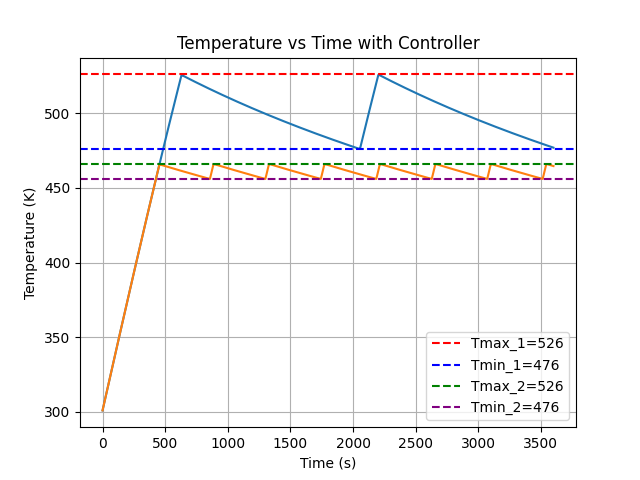
\includegraphics[width=0.8\textwidth]{imgs/heater_w._controll_3.png}  % Вставка изображения
	\caption{Моделирование для 
		\[
		P=35\text{Вт}, m = 0.25\text{кг}, c=375\frac{\text{Дж}}{\text{кг}\cdot\text{К}},k = 2, S = 0.00094 \text{м}^2,T_{env}= 296 \text{К}
		\].}  % Подпись к изображению
	\label{fig:heater_with_controll_3}  
\end{figure}
\newpage
\begin{figure}[h]  % Окружение для картинки
	\centering
	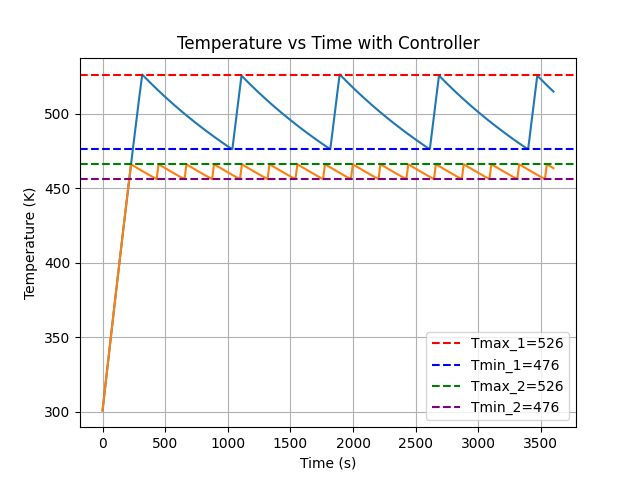
\includegraphics[width=0.8\textwidth]{imgs/heater_w._controll_2.png}  % Вставка изображения
	\caption{Моделирование для 
		\[
		P=35\text{Вт}, m = 0.25\text{кг}, c=180\frac{\text{Дж}}{\text{кг}\cdot\text{К}},k = 2, S = 0.00094 \text{м}^2,T_{env}= 296 \text{К}
		\].}  % Подпись к изображению
	\label{fig:heater_with_controll_2}  
\end{figure}
\begin{figure}[h]  % Окружение для картинки
	\centering
	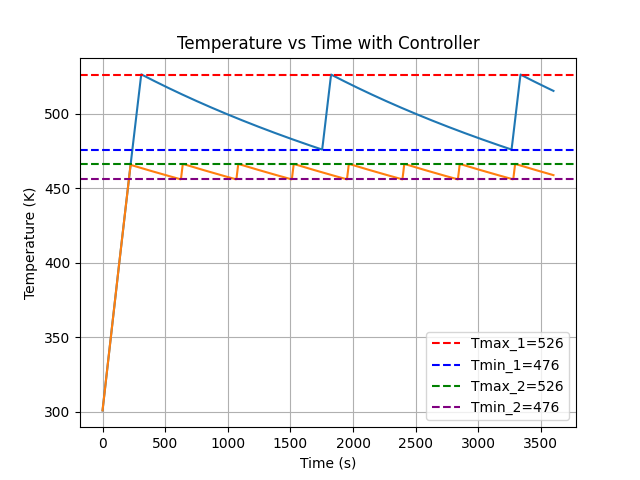
\includegraphics[width=0.8\textwidth]{imgs/heater_w._controll_1.png}  % Вставка изображения
	\caption{Моделирование для 
		\[
		P=70\text{Вт}, m = 0.25\text{кг}, c=375\frac{\text{Дж}}{\text{кг}\cdot\text{К}},k = 2, S = 0.00094 \text{м}^2,T_{env}= 296 \text{К}
		\].}  % Подпись к изображению
	\label{fig:heater_with_controll_1}  
\end{figure}
\newpage
На рис. \ref{fig:heater_with_controll_3} -  \ref{fig:heater_with_controll_1} показано, что при достижении максимальной температуры, нагревательный элемент отключается, благодаря работе контроллера. Аналогично, при достижении минимальной температуры нагреватель включается, и температура растёт.